\edtext{\edlabel{4143r1}}{\lemma{\textso{4.}}\xxref{4143r1}{4143r2}\Afootnote{ \textit{ (1) }\ Pour moy s'il m'est permis, de dire ma pens\'{e}e, quoyque toutes les experiences projett\'{e}es ne soyent pas faites encor \textit{ (2) }\ Un de mes amis avoit cette pensée, que \textit{(a)}\ la pesanteur \textit{(b)}\ l'atmosphere pese sur les placques dans le vuide même faisant entrer par les pores du verre, des ruisseaux d'un air subtil et rafiné. Mais \textit{(aa)}\ \`{a} \textit{(bb)}\ si cela \textit{(cc)}\ cela expliqueroit seulement le phenomene des placques, car si cette pression de l'atmosphere estoit veritable les liqueurs non purg\'{e}es ne tomberoient pas dans le vuide, et une petite bulle d'air dont l'effort n'est point considerable, \`{a} l'\'{e}gard de l'atmosphere, ne les d\'{e}tacheroit non plus.  \textit{ (3) }\ Ce sera peut estre \textit{ (4) }\ Le [...] estre \textit{ L}}}\pend
\clearpage
\pstart [143 v\textsuperscript{o}] Le dernier ressort, sera peut estre, apres avoir essay\'{e} tout en vain,\linebreak \vspace{-10pt}d'avoir recours en partie \`{a} l'explication des anciens \edtext{\edlabel{4143r2}qui estoit en usage}{\lemma{}\Afootnote{qui estoit en usage \textit{ erg.} \textit{ L}}}, devant qu'on a entendu parler de l'experience de Torricelli\protect\index{Sachverzeichnis}{exp\'{e}rience de Torricelli} et de la machine de Mons. Guericke\protect\index{Namensregister}{\textso{Guericke} (Gerickius, Gerick.), Otto v. 1602\textendash 1686}. S\c{c}avoir que deux placques\protect\index{Sachverzeichnis}{deux placques} ne peuuent estre separ\'{e}es, \edtext{m\^{e}me dans le Recipient \'{e}puis\'{e};}{\lemma{m\^{e}me}\Afootnote{dans le  \textit{ (1) }\ vuide\protect\index{Sachverzeichnis}{ vuide|textit} \textit{ (2) }\ Recipient \'{e}puis\'{e}; \textit{ erg.} \textit{ L}}} ny les liqueurs purg\'{e}es\protect\index{Sachverzeichnis}{liqueur!purg\'{e}e}, d\'{e}tach\'{e}es du tuyau; sans qu'une matiere remplisse en m\^{e}me temps l'espace \edtext{entre deux placques\protect\index{Sachverzeichnis}{deux placques}, ou entre la liqueur et la superficie interieure du tuyau ou de la phiole:}{\lemma{}\Afootnote{entre deux placques\protect\index{Sachverzeichnis}{deux placques}, ou  \textit{ (1) }\ dans le tuyau \textit{ (2) }\ entre [...] phiole: \textit{ erg.} \textit{ L}}} qui demeureroit vuide sans cela, soit que ce doiuue estre un air subtil, ou que ce soit une matiere fluide etherienne\protect\index{Sachverzeichnis}{mati\`{e}re!fluide etherienne}; laquelle neantmoins trouue quelque difficult\'{e} \`{a} passer par les pores des placques, ou des vases. 
\edtext{Et c'est la nouuelle pression conforme \`{a} celle dont \textso{Monsieur }\textso{Huguens}\protect\index{Namensregister}{\textso{Huygens} (Hugenius, Vgenius, Hugens, Huguens), Christiaan 1629\textendash 1695}, auquel nous sommes redeuuables de la demonstration d'une verit\'{e} si importante, parle dans le \textit{Journal des S\c{c}avants}.}{\lemma{}\Afootnote{Et c'est la nouuelle pression   \textbar\ conforme \`{a} celle \textit{ erg.}\ \textbar\  dont [...] \textit{Journal des S\c{c}avants}. \textit{ erg.} \textit{ L}}}\edtext{}{\lemma{\textit{S\c{c}avants}.}\Bfootnote{\textsc{Chr. Huygens, }\cite{00062}\textit{Extrait d'une lettre}, \textit{JS} (1672), S.~140. (\textit{HO}, VII, S.~206).}} Mais toute la \edtext{peine}{\lemma{la}\Afootnote{ \textit{ (1) }\ difficult\'{e} \textit{ (2) }\ peine \textit{ L}}} sera d'expliquer, \edtext{pourquoy il faut que le corps suspendu soit purg\'{e} d'air, et comment par apres}{\lemma{d'expliquer,}\Afootnote{ \textit{ (1) }\ comment \textit{ (2) }\ pourquoy [...] et \textit{(a)}\ pourquoy \textit{(b)}\ comment par apres \textit{ L}}} une petite bulle d'air n\'{e}e dans le tuyau plein de la liqueur purg\'{e}e\protect\index{Sachverzeichnis}{liqueur!purg\'{e}e}, facilite le passage \edtext{\`{a} ce fluide}{\lemma{}\Afootnote{\`{a} ce fluide \textit{ erg.} \textit{ L}}}, pour faire tomber la liqueur, \edlabel{143va}personne n'ayant expliqu\'{e} pourquoy ce fluide subtil\protect\index{Sachverzeichnis}{fluide!subtil} doit enfler cette bulle, et ne peut sans cela remplir la place que la liqueur doit quitter. Car de dire que la bulle ou le fluide qui est dedans elle contient un certain effort, \'{e}gale \`{a} celuy qui so\^{u}tient la liqueur purg\'{e}e\protect\index{Sachverzeichnis}{liqueur!purg\'{e}e}, cela ne se peut nullement expliquer, partout; ce qu'on a mis en oeuure jusqu'à là, comme j'ay montré déja cy dessus. Car il n'est pas necessaire que la Bulle égale tousjours l'air du Recipient: de plus l'air du Recipient ne soûtient pas la liqueur et le mouuement des fluides en tous sens est incapable de faire une pression égale de deux costez, la quantité des coups n'estant pas égale, comme il est necessaire pour cet effect, sans que l'ouuerture de deux costez soit égale, ce qui ne se trouue pas icy, la bulle pouuant estre moindre que la bouche de la phiole. Mais, dira-t-on la pression du fluide subtil dans la bulle d'air, égale pourtant celle du même fluide dans l'air qui reste au Recipient, la pression à present estant de deux costez sur la liqueur suspendüe même selon l'hypothese que nous venons d'approuuer. Il est vray, mais c'est aussi la question pourquoy ce fluide subtil, qui passe asseurement par le verre et la liqueur purgée, aussi bien que par la bulle d'air (puisqu'il faut qu'il passe neantmoins par le verre, pour entrer dans la bulle) ne presse pas sur la liqueur purgée, si non par la bulle. Et cette question resteroit tousjours, si même ce qu'on avoit avancé touchant le mouuement des fluides en tous sens,  pour en tirer la raison de nos phenomenes, pourroit estre \edlabel{143ve} \edtext{soûtenu.}{\lemma{personne}\xxref{143va}{143ve}\Afootnote{ [...] bulle  \textbar\ ou [...] elle \textit{ erg.}\ \textbar\  contient [...] expliquer, \textit{ (1) } au moins \textit{ (2) } partout; [...] égale \textbar\ tousjours \textit{ erg.} \textbar\ l'air [...] égale, \textbar\ comme [...] effect, \textit{ erg.} sans [...] phiole. \textit{ erg.} \textbar\ Mais, [...] bulle \textbar\ d'air \textit{ erg.} \textbar\ égale \textbar\ pourtant \textit{ erg.} \textbar\ celle [...] Recipient, \textit{ (a) } c'est vray \textit{ (b) } la [...] costez \textbar\ sur [...] d'approuuer. \textit{ erg.} Il [...] passe \textbar\ asseurement \textit{ erg.} \textbar\ par \textit{ (aa) } l'eau et le verse \textit{ (bb) } le [...] d'air \textit{ (aaa) } (car si l'on me le nie, je le pranuerois par une experience \textit{ (bbb) } ne presse pas la liqueur \textit{ (ccc) } (puisqu'il [...] sens, \textit{ (aaaa) } poursoit estre soûtenu \textit{ (bbbb) } pour en rendre raison de nos phenomenes \textit{ (cccc) } pour [...] soûtenu. \textit{ erg.} \textit{ L}}}
 \edtext{Comme donc c'est le noeud de la question, voila ce que j'ay trouu\'{e} jusqu' \`{a} l\`{a} de plus vraysemblable pour developper cette difficult\'{e}: je crois donc, qu'on sera peut estre oblig\'{e}, de dire, que ce fluide subtil}{\lemma{soûtenu.}\Afootnote{ \textit{ (1) }\ On sera donc oblig\'{e} peut estre de dire, que la dite matiere fluide\protect\index{Sachverzeichnis}{mati\`{e}re!fluide|textit} \textit{ (2) }\ Comme   \textbar\ donc \textit{ erg.}\ \textbar\ c'est [...] vraysemblable  \textbar\ pour developper cette difficult\'{e} \textit{ erg.}\ \textbar\ : je [...] subtil \textit{ L}}}, ne se peut remuer, ais\'{e}ment,  que dans l'air, ou autre corps sensible\protect\index{Sachverzeichnis}{corps!sensible}; ayant de la peine d'entrer dans un lieu \edtext{vuide. Et \`{a} fin qu'on ne prenne pas cela pour une pure supposition en l'air, je le confirme par une experience toute faite mille fois, laquelle quoyqu'elle sera peut estre jug\'{e}e d'abord \'{e}loign\'{e}e de nostre affaire; contentera peut estre les esprits estant approfondie. Je le confirme donc}{\lemma{vuide}\Afootnote{ \textit{ (1) }\ sans cela. Ce qui se confirme \textit{ (2) }\ . Et [...] affaire; \textit{(a)}\ j'espere pourtant \textit{(b)}\ contentera [...] donc \textit{ L}}} par la nature surprenante de la lumiere, 
    %Bild ans Ende gesetzt
  %         \begin{wrapfigure}{l}{0.3\textwidth}                    
      %          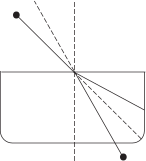
\includegraphics[width=0.3\textwidth]{images/37_3_143v1}\\\textit{[Fig. 6, Zeichnung auf Bl. 134r\textsuperscript{o}]}
                        %\caption{Bildbeschreibung}
          %              \end{wrapfigure}
                        %@ @ @ Dies ist eine Abstandszeile - fuer den Fall, dass mehrere figures hintereinander kommen, ohne dass dazwischen laengerer Text steht. Dies kann zu einer Fahlermeldung fuehren. @ @ @ \\ vuide.
           les phenomenes de la refraction\protect\index{Sachverzeichnis}{r\'{e}fraction} nous faisant voir, que les rayons \edtext{passent}{\lemma{rayons}\Afootnote{ \textit{ (1) }\ entrent \textit{ (2) }\ passent \textit{ L}}} avec plus de difficult\'{e} par une matiere moins grossiere, s'ecartant d'avantage de la perpendiculaire quand ils \edtext{sortent de l'eau ou du verre, dans l'air, que quand ils entrent de l'air dans l'eau}{\lemma{ils}\Afootnote{ \textit{ (1) }\ entrent dans l'air, \textit{ (2) }\ sortent [...] ils \textit{(a)}\ rencontrent l'eau \textit{(b)}\ entrent de l'air dans l'eau \textit{ L}}} ou verre; \edtext{duquel phenomene embarass\'{e} jusqu'\`{a} l\`{a} je crois}{\lemma{}\Afootnote{duquel [...] crois \textit{ erg.} \textit{ L}}} avoir trouu\'{e} une demonstration nouuelle toute claire et mecanique, que je proposeray \edtext{ailleurs.}{\lemma{ailleurs.}\Bfootnote{Vgl. N.21.}} Le fait cependant, estant pos\'{e} pourquoy n'oserions nous pas dire, \edtext{qu'un tel fluide subtil, insensible entre avec plus de peine dans les matieres sensibles les plus}{\lemma{dire,}\Afootnote{ \textit{ (1) }\ que le fluide subtil\protect\index{Sachverzeichnis}{fluide!subtil|textit}, qui passe avec plus de peine les  \textit{(a)}\ corps pl \textit{(b)}\ matieres \textit{ (2) }\ qu'un [...] plus \textit{ L}}} subtiles; \edtext{et}{\lemma{et}\Afootnote{ \textbar\ entre \textit{ gestr.}\ \textbar\ avec \textit{ L}}} avec grandissime les lieux vuides, ou d\'{e}pourveus de tout le corps\protect\index{Sachverzeichnis}{corps!sensible} grossier ou sensible, voire de l'air m\^{e}me. \edtext{Donc ce fluide}{\lemma{Donc}\Afootnote{ \textit{ (1) }\ la matiere \textit{ (2) }\ ce fluide \textit{ L}}} subtil quoyqu'il puisse passer par le verre et par l'eau, ne pourra pas \edtext{ais\'{e}ment}{\lemma{}\Afootnote{ais\'{e}ment \textit{ erg.} \textit{ L}}} remplir incontinent l'espace quitt\'{e} \edtext{par la placque inferieure ou la liqueur purg\'{e}e\protect\index{Sachverzeichnis}{liqueur!purg\'{e}e} quand elles tombent, s'il ne s'y trouue point d'air, ou autre corps sensible\protect\index{Sachverzeichnis}{corps!sensible} qui succede. Au reste il est assez evident, pourquoy la bulle ne fait tomber la liqueur purg\'{e}e\protect\index{Sachverzeichnis}{liqueur!purg\'{e}e}, qu'estant arriv\'{e} au point \textit{B}. (\textso{fig. }[\textso{1}]\edtext{}{\Afootnote{\textso{4}\textit{\ L \"{a}ndert Hrsg.}}}\textso{.}) c'est \`{a} dire \`{a} l'espace \textit{CD-B} qu'elle pourra remplir, apres que la liqueur sera tomb\'{e}e (la nature n'entreprennant rien au dela de ses forces.) Car la partie de la liqueur purg\'{e}e\protect\index{Sachverzeichnis}{liqueur!purg\'{e}e} \textit{AB} estant \textso{so\^{u}ten\"{u}e} par le ressort\protect\index{Sachverzeichnis}{ressort} de l'air qui reste dans le Recipient \textit{EE} et la partie \textit{CD-B} estant \textso{suspendue} par la force unitive: la bulle d'air, comme elle n'a rien a d\'{e}m\^{e}ler avec l'air du Recipient \textit{EE} (l'espace \textit{CD-B} estant assez grand pour la loger, \`{a} moins qu'elle, l'ayant rempli ne se trouueroit trop contrainte et moins dilat\'{e}e que l'air du Recipient, qui par consequent en ce cas, cederoit un peu, et le point \textit{B} tomberoit au dessous de la hauteur que le ressort\protect\index{Sachverzeichnis}{ressort} de l'air du Recipient peut so\^{u}tenir) ne commence d'agir, qu'estant arriv\'{e}e, \`{a} la partie de la liqueur, suspend\"{u}e par la force unitive dont l'effect a dependu entierement de l'absence de la bulle, puisqu'il faut que la liqueur pour estre suspend\"{u}e (autrement que par la pression de l'air, trouu\'{e}e par Torricelli\protect\index{Namensregister}{\textso{Torricelli} (Torricellius), Evangelista 1608\textendash 1647},) soit purg\'{e}e d'air. Ce n'est pas donc merveille, qu' \`{a} l'arriv\'{e}e de la bulle, la liqueur tombe. ⟨−⟩ Je pourrois donc finir icy si je ne me trouuois oblig\'{e} de faire auparavant une remarque de consequence pour toute la philosophie naturelle; car}{\lemma{}
           \Afootnote{par [...] qu'elle, \textit{ (1) }\ ne soit \textit{ (2) }\ l'ayant [...] consequent  \textbar\ en ce cas, \textit{ erg.}\ \textbar\ cederoit [...] suspendüe \textit{ (a) } autrement que par la pression de l'air, \textit{ (b) }(autrement que par la pression de l'air, trouu\'{e}e par Torricelli\protect\index{Namensregister}{\textso{Torricelli} (Torricellius), Evangelista 1608\textendash 1647},) soit [...] car \textit{ erg.} \textit{ L}}} 
           %laliqueur purg\'{e}e\protect\index{Sachverzeichnis}{liqueur!purg\'{e}e}quand [...] autrecorps sensible\protect\index{Sachverzeichnis}{corps!sensible}qui [...] laliqueur purg\'{e}e\protect\index{Sachverzeichnis}{liqueur!purg\'{e}e}, qu'estant arriv\'{e} au point \textit{B}. (\textso{fig. }[\textso{1}]\edtext{}{\Afootnote{\textso{4}\textit{\ L \"{a}ndert Hrsg. } }}\textso{.}) @@@ G R A F I K @@@ c'est \`{a} dire \`{a} l'espace \textit{CD-B}qu'elle [...] laliqueur purg\'{e}e\protect\index{Sachverzeichnis}{liqueur!purg\'{e}e} \textit{AB} estant \textso{so\^{u}ten\"{u}e} par le ressort\protect\index{Sachverzeichnis}{ressort}de [...] Recipient\textit{EE} et la partie \textit{CD-B} estant \textso{suspendue}par [...] Recipient\textit{EE} (l'espace \textit{CD-B}estant [...] qu'elle, \textit{ (1) }\ ne soit \textit{ (2) }\ l'ayant rempli ne se trouueroittrop [...] consequent  \textbar\ en ce cas, \textit{ erg.}\ \textbar\  cederoit un peu, et le point \textit{B} tomberoit au dessous de la hauteur que le ressort\protect\index{Sachverzeichnis}{ressort} de l'air du Recipient peut so\^{u}tenir) ne commence d'agir, qu'estant arriv\'{e}e, \`{a} la partie de la liqueur, suspend\"{u}e par la force unitive dont l'effect a dependu entierement de l'absence de la bulle, puisqu'il faut que la liqueur pour estre suspend\"{u}e (autrement que par la pression de l'air,  \textbar\ trouu\'{e}e par Torricelli\protect\index{Namensregister}{\textso{Torricelli} (Torricellius), Evangelista 1608\textendash 1647},) \textit{ erg.}\ \textbar\  soit purg\'{e}e d'air. Ce n'est pas donc merveille, qu' \`{a} l'arriv\'{e}e de la bulle, la liqueur tombe. ⟨−⟩ Je pourrois donc finir icy si je ne me trouuois oblig\'{e} de faire auparavant une remarque de consequence pour toute la philosophie naturelle; car \textit{ erg.} \textit{ L}}} 
           comme il y a des philosophes, qui font difficult\'{e}, et pas tout \`{a} fait sans raison, d'avo\"{u}er des pores dans le verre ou autres corps solides\protect\index{Sachverzeichnis}{corps!solide} \edtext{sans que l'experience les y oblige absolument}{\lemma{}\Afootnote{sans [...] absolument \textit{ erg.} \textit{ L}}} \edtext{il est bon d'admoneter qu'il y a}{\lemma{absolument}\Afootnote{ \textit{ (1) }\ il y a \textit{ (2) }\ il est bon d'admoneter qu'il y a \textit{ L}}} icy de quoy leur satisfaire aussi, en tournant un peu la facon de parler\edtext{, et en se servant}{\lemma{parler}\Afootnote{ \textit{ (1) }\ . Car cela pos\'{e}, il faut \textit{(a)}\ dire \textit{(b)}\ se servir \textit{ (2) }\ , et en se servant \textit{ L}}} de la propagation des pressions ou efforts au lieu du passage d'un fluide subtil\protect\index{Sachverzeichnis}{fluide!subtil}. \edtext{Un lieu vuide c'est \`{a} dire sans autre effort ou impression que celle qu'on luy va donner à present, estant incapable d'en recevoir, que des momentan\'{e}es ou passageres; les veritables ou effectifs, ne se fixant que par une resistence des pressions ou efforts qui se trouuent d\'{e}ja dans ce lieu. Car d'ailleurs, on trouuera}{\lemma{subtil.}\Afootnote{ \textit{ (1) }\ Et peut \textit{ (2) }\ Il se trouuera \textit{ (3) }\ Un lieu vuide   \textbar\ c'est à dire sans autre \textit{ (1) }\ pression \textit{ (2) }\ effort ou impression que celle \textit{ (a) }\ il va recevoir \textit{ (b) }\ qu'on luy va donner à present, \textit{ erg.}\ \textbar\  estant incapable d'en recevoir,  \textbar\ si ce n'est \textit{ erg. u.}\  \textit{ gestr.}\ \textbar\ que [...] pressions  \textbar\ ou efforts \textit{ erg.}\ \textbar\ qui [...] trouuera \textit{ L}}} peut estre, que le m\^{e}me moyen suffira \`{a} nous desembarrasser  de toutes les difficult\'{e}s de la rarefaction et condensation sans \edtext{employer}{\lemma{sans}\Afootnote{ \textit{ (1) }\ supposer \textit{ (2) }\ employer \textit{ L}}} l'interposition d'une matiere subtile\protect\index{Sachverzeichnis}{mati\`{e}re!subtile} \edtext{qui passe par les pores des corps}{\lemma{}\Afootnote{qui [...] corps \textit{ erg.} \textit{ L}}}: Surtout si la nature du corps\protect\index{Sachverzeichnis}{nature du corps}, ou de la Matiere, consiste dans le Mouuement ou Effort, au lieu de l'Extension, comme il y a de l'apparence. Par consequent la condensation ne sera qu'une augmentation, et la rarefaction ne sera qu'une diminuation des \edtext{Efforts; une certaine quantit\'{e} de matiere, c'est \`{a} dire}{\lemma{Efforts;}\Afootnote{ \textit{ (1) }\ plus matiere, c'est \`{a} dire plus \textit{ (2) }\ une [...] dire \textit{ L}}} d'effort, estant tantost repand\"{u}e par un grand espace, tantost concentr\'{e}e dans un petit, sans qu'on doiuue \edtext{plus avoir peur de ces deux grands phant\^{o}mes d'une philosophie peu fond\'{e}e: de la \textso{penetration des dimensions}}{\lemma{doiuue}\Afootnote{ \textit{ (1) }\ avoir   \textbar\ de la penetration des dimensions peur \textit{ erg.}\ \textbar\  \textit{ (2) }\ plus [...] phant\^{o}mes \textit{(a)}\ de la philosophie mal fond\'{e}e \textit{(b)}\ d'une philosophie  \textit{(aa)}\ peu asseur\'{e}e  \textit{(bb)}\ peu [...] \textso{dimensions} \textit{ L}}} \edtext{(que quelques uns ont cr\"{u}e impossible, m\^{e}me au Toutpuissant. La question s'estant \'{e}chauff\'{e}e \`{a} l'occasion des controverses de l'Eucharistie)}{\lemma{}\Afootnote{(que [...] l'Eucharistie) \textit{ erg.} \textit{ L}}} \edtext{et \textso{du Vuide}}{\lemma{l'Eucharistie)}\Afootnote{ \textit{ (1) }\ pour la condensation, et \textso{du }\textso{Vuide}\protect\index{Sachverzeichnis}{vide|textit} \textit{ (2) }\ pour la rarefaction \textit{ (3) }\ et \textso{du Vuide} \textit{ L}}}. Mais \edtext{plus de loisir, necessaire \`{a} une examination meure et rigoureuse, nous fera juger}{\lemma{plus}\Afootnote{[...] juger \textit{ erg.} \textit{ L}}} si cette opinion, dont je crois parler le premier, a autant de solidit\'{e} qu'elle a de l'apparence.\pend 
     %          \begin{center}                    
         %       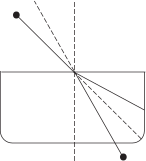
\includegraphics[width=0.3\textwidth]{images/37_3_143v1}\\\textit{[Fig. 6, Zeichnung auf Bl. 134r\textsuperscript{o}]}
                        %\caption{Bildbeschreibung}
             %           \end{center}